\documentclass[11pt]{article}

% Document config
\usepackage[letterpaper, margin=1in]{geometry}
\usepackage[utf8]{inputenc}
\usepackage[spanish]{babel}
\usepackage{tikz}
\usepackage{url}
\usepackage{amsmath}
\usepackage{graphicx}
\bibliography{biblist}  % Biliografía
\usepackage{color}
\usepackage{xcolor}
\usepackage{float}
\usepackage{tcolorbox}
\usepackage{biblatex} %Imports biblatex package
\addbibresource{biblist.bib} %Import the bibliography file

\usepackage[framed, numbered]{listings}
\lstdefinestyle{customc}{
  belowcaptionskip=1\baselineskip,
  breaklines=true,
  frame=L,
  xleftmargin=\parindent,
  language=C,
  showstringspaces=false,
  basicstyle=\footnotesize\ttfamily,
  keywordstyle=\bfseries\color{cyan},
  commentstyle=\itshape\color{orange},
  identifierstyle=\color{violet},
  stringstyle=\color{teal},
}

\lstset
{ %Formatting for code in appendix
    language=C,
    keywordstyle=\bfseries\color{magenta},
    commentstyle=\itshape\color{orange},
    identifierstyle=\color{teal},
    stringstyle=\color{teal},
    basicstyle=\footnotesize,
    numbers=left,
    stepnumber=1,
    showstringspaces=false,
    tabsize=1,
    breaklines=true,
    breakatwhitespace=false,
    frame=single
}

% Color definitions
\definecolor{darkblue}{rgb}{0 , 0.054 , 0.196}
\definecolor{mygreen}{rgb}{0,0.6,0}
\definecolor{mygray}{rgb}{0.8,0.8,0.8}
\definecolor{codeBG}{rgb}{0.9, 0.97, 0.9}
\definecolor{mymauve}{rgb}{0.58,0,0.82}

\addto\captionsspanish{% Replace "english" with the language you use
  \renewcommand{\contentsname}%
    {Tabla de contenidos}%
}

\title{
{
    \begin{tikzpicture}[overlay, remember picture]
        \node[anchor=north west, %anchor is upper left corner of the graphic
            xshift=3cm, %shifting around
            yshift=-4cm]
            at (current page.north west) %left upper corner of the page
        {
\includegraphics[height=2cm]{./imagenes/EIE.png}};
    \end{tikzpicture}
    \begin{tikzpicture}[overlay, remember picture]
        \node[anchor=north east, %anchor is upper left corner of the graphic
            xshift=-1.5cm, %shifting around
            yshift=-4cm]
            at (current page.north east) %left upper corner of the page
        {
\includegraphics[height=2cm]{./imagenes/UCR_logo.png}};
    \end{tikzpicture}
    \Large
        \textbf{Universidad de Costa Rica}\\
        Facultad de Ingeniería\\
        Escuela de Ingeniería Eléctrica\\~\\
        \texttt{IE-0117} Programación bajo plataformas abiertas
    }
    ~\\~\\
    {\LARGE Proyecto Final: AuVeTA, \\ Autonomous Vehicle for Tracking and Control Aplications.}
}
\author{Jorge Isaac Fallas Mejía B62562\\
Esteban Rodríguez Quintana B66076\\
Fabio Villalobos Pacheco B78346}

\date{I-2019}




\begin{document}
\maketitle


\hrule
\hrule
\tableofcontents
\hspace{5mm}
\hrule
\hrule

\section{Reseña del proyecto a implementar}

El proyecto AuVeTA consiste en diseñar y poner en funcionamiento un vehículo que pueda ser utilizado como una base para prototipado de un vehículo que a futuro pueda utilizarse en aplicaciones de seguimiento de linea para algún tipo de aplicación industrial o inclusive evolucionar al mundo del reconocimiento de patrones y la visión por computador para generar una propuesta de vehículos realmente autónomos y con aplicación enfocada a la movilidad humana.

Este proyecto consiste en el desarrollo de un vehículo semi autónomo que, mediante la implementación de microcontroladores, sensores, un módulo de comunicación y programación, pueda cumplir con el objetivo de seguir una línea de color en el suelo y llegar a un punto donde culmine con la ejecución de una tarea determinada. Parte de las funciones que se desean incorporar a este prototipo, además del seguimiento de línea y remoción de obstáculos, son la comunicación del vehículo con un centro de control, desde el cual también se pueda conducir a discreción el mismo, con la finalidad de ser utilizado en otro tipo de aplicaciones mediante sus distintos modos de operación.

El proyecto consta de dos partes principales: hardware y software. El desarrollo e integración de estos dos subsistemas han de ir de la mano, puesto que un error en uno de ellos ha de limitar la acción correcta del otro.
\newpage
\section{Funcionamiento del programa}
\subsection{Funcionamiento de Software}

El código se implementará en dos etapas, la primera consiste en una etapa de control y la segunda en una etapa de seguimiento, ambas son completamente independientes la una de la otra.

\begin{itemize}
    \item \textbf{Seguimiento}: La etapa de seguimiento implementa el sensor de línea, la idea es regular el funcionamiento de los motores de acuerdo a la corrección que ha de ser necesario para mantener el vehículo encima de la línea a seguir, y garantizar de esta forma seguimiento del trazo deseado. Toda la implementación de este código se hará programada en el IDE de Arduino puesto que al ser la etapa semi autónoma del proyecto no requiere de ningún comando desde un centro de control para la toma de decisiones. 
    Esta etapa de seguimiento implementa 3 sensores, uno para reconocer la línea a seguir, y dos sensores de obstáculo, uno de ellos encargado de detectar obstáculos frente al vehículo para su remoción, y el otro sensor para reconocer cuando se llega al final del recorrido.
    
    \item \textbf{Control}: La etapa de control se encarga de manejar el funcionamiento de los motores de manera remota mediante un módulo bluetooth, la idea es enviar datos desde un programa en C a través del puerto serial. Dependiendo de qué dato sea enviado, el vehículo llevará a cabo distintos movimientos. El programa en C cuenta con distintas funciones que permiten controlar el puerto serial, al cual se conecta el módulo bluetooth, son dos funciones en total. La primera se encarga de inicializar el puerto serial, una vez inicializado se puede utilizar la otra función, que se utiliza para escribir en el puerto serial, de esa forma se establece una comunicación unidireccional. Dichas funciones serán implementadas en una interfaz gráfica que simula un control remoto, la idea es controlar el vehículo con el teclado, y con la interfaz visualizar los movimientos que realiza el vehículo.
\end{itemize}

\subsubsection{Interfaz}
La interfaz utilizada en este proyecto utiliza una herramienta llamada GTK, más específicamente GTK+-2.0, la cual es una multiplataforma de herramientas que permite crear interfaces de gráficas de uso para el usuario. Este ofrece un set completo de widgets, estos siendo pequeñas aplicaciones con accesos directos permitiendo la sencilla visualización de las funciones principales utilizadas en determinado programa o documento. También es adaptable a proyectos que van desde pequeñas herramientas hasta aplicaciones muy completas permitiendo su funcionalidad. Se usa en diferentes sistemas operativos tales como Windows, GNU/Linux and Unix, OSX e inclusive dispositivos móviles. Escrito en lenguaje C, y permitido además en C++, Perl y Python. \cite{interfaz}
    \begin{itemize}
        \item\textbf{Función para crear las características del botón:}
        Esta es la función tipo Gtkwidget que recibe que la tabla o matriz interna se establecerá en la ventana de la interfaz que contendrá los botones, un dato char que es el tamaño de los botones, además dos datos de  tipo int que son la posición en fila y columna de los botones, luego esta hace un gtk button new with label que es el botón, además del color, de la posicion en la interfaz y  gtk widget show que hace que retorne todas esas características del botón.
        
\begin{lstlisting}

GtkWidget *CreateButton(GtkWidget *table, char *szLabel, int row, int column)
{
        GtkWidget *button;

        button = gtk_button_new_with_label(szLabel);

        gtk_signal_connect(GTK_OBJECT(button), "clicked",
                           GTK_SIGNAL_FUNC(button_clicked), szLabel);

        GdkColor color;

        gdk_color_parse("red", &color);

        gtk_widget_modify_bg(GTK_WIDGET(button), GTK_STATE_NORMAL, &color);

        gtk_table_attach(GTK_TABLE(table), button,
                         column, column + 1,
                         row, row + 1,
                         GTK_FILL | GTK_EXPAND,
                         GTK_FILL | GTK_EXPAND,
                         10, 15);

        gtk_widget_show(button);

        return (button);
}
\end{lstlisting}
        \item\textbf{Función que crea el botón en la interfaz:}
        Esta función es de tipo void que recibe la tabla o matriz interna, se establecerá en la ventana de la interfaz que contendrá los botones, luego se crea un dato que hace que el ciclo for recorra la lista de los botones y con ayuda de la función CreateButton se cree el botón y aparezca en la interfaz.
        
\begin{lstlisting}
void CreateControlButtons(GtkWidget *table)
{
        int nIndex;

        for (nIndex = 0; nIndex < numbuttons; nIndex++)
        {

                buttonList[nIndex].widget =
                    CreateButton(table,
                                 buttonList[nIndex].szLabel,
                                 buttonList[nIndex].row,
                                 buttonList[nIndex].col);
        }
}
\end{lstlisting}

 \item\textbf{Función para poder usar los botones del teclado:}
        Esta función es de tipo void que recibe un widget, un evento y la información del teclado, hace uso de un ciclo for que da busqueda entre los botones, y una condición if que permite si la pulsación de la tecla es el primer carácter de un botón y la longitud de la etiqueta del botón es de 1, entonces permite el retorno que conecta el botón presionado en el teclado con la interfaz gráfica y la tarea asociada.
    

\begin{lstlisting}
void key_press(GtkWidget *widget,
               GdkEventKey *event,
               gpointer data)
{
        int npressed;

        for (npressed = 0; npressed < numbuttons; npressed++)
        {
                if (event->keyval == buttonList[npressed].szLabel[0] &&
                    buttonList[npressed].szLabel[1] == (char)0)
                {
                        gtk_widget_grab_focus(buttonList[npressed].widget);
                        gtk_button_clicked(GTK_BUTTON(buttonList[npressed].widget));
                        return;
                }
        }
}

\end{lstlisting}

        \item\textbf{Función para clickear el botón y realizar una tarea:}
        Es la función de tipo void que recibe un widget y la información, este contiene dos datos tipo int los cuales son el baud rate y el puerto, dos punteros de tipo char, el str se encarga de agarrar el texto del botón y la información, además contiene la ventana que contiene la interfaz, luego varias condiciones if que permiten comparar el botón clickeado o presionado en el teclado que conecta con el puerto serial y retorna la tarea que realiza el vehículo. 
        
\begin{lstlisting}
void button_clicked(GtkWidget *widget, gpointer data)
{
        int baudrate = 115200;
        int port;
        port = serialport_init("/dev/rfcomm0", baudrate);

        char ch = *((char *)data);
        char *str;
        GtkWidget *window;
        window = gtk_window_new(GTK_WINDOW_TOPLEVEL);

        str = (char *)data;

        if (strcmp(str, "w") == 0)
        {

                char a = 'w';
                const char *ptr = &a;
                serialport_write(port, ptr);

                return;
        }
        else if (strcmp(str, "a") == 0)
        {

                char a = 'a';
                const char *ptr = &a;
                serialport_write(port, ptr);

                return;
        }
        else if (strcmp(str, "d") == 0)
        {

                char a = 'd';
                const char *ptr = &a;
                serialport_write(port, ptr);

                return;
        }
        else if (strcmp(str, "s") == 0)
        {

                char a = 's';
                const char *ptr = &a;
                serialport_write(port, ptr);

                return;
        }
        else if (strcmp(str, "1") == 0)
        {

                char a = '1';
                const char *ptr = &a;
                serialport_write(port, ptr);

                gtk_label_set(GTK_LABEL(label), "Control Mode");
                return;
        }
        else if (strcmp(str, "2") == 0)
        {

                char a = '2';
                const char *ptr = &a;
                serialport_write(port, ptr);

                gtk_label_set(GTK_LABEL(label), "Waiting mode");
                return;
        }
        else if (strcmp(str, "3") == 0)
        {

                char a = '3';
                const char *ptr = &a;
                serialport_write(port, ptr);

                gtk_label_set(GTK_LABEL(label), "Tracking mode");
                return;
        }
        else if (strcmp(str, "y") == 0)
        { //scalubur time

                char a = 'e';
                const char *ptr = &a;
                serialport_write(port, ptr);

                return;
        }
        else if (strcmp(str, "b") == 0)
        { //buzzer

                char a = 'b'; 
                const char *ptr = &a;
                serialport_write(port, ptr);

                return;
        }
        else if (strcmp(str, "t") == 0)
        { //trompo

                char a = 't';
                const char *ptr = &a;
                serialport_write(port, ptr);

                return;
        }

      
}
\end{lstlisting}

        \item\textbf{Función para cerrar la ventana y finalizar el programa:}
        Es una función de tipo int que recibe un widget y la información, que utiliza un gtk main quit que retorna el cierre de la ventana y, por ende, del programa.
        
\begin{lstlisting}
int CloseAppWindow(GtkWidget *widget, gpointer data)
{
        gtk_main_quit();

        return (FALSE);
}
\end{lstlisting}
        
    \end{itemize}   
   

\subsubsection{Comunicación}
La comunicación cuenta con varios elementos fundamentales.
\begin{itemize}
    \item\textbf{Módulo bluetooth HC-05:} El módulo bluetooth permite establecer una comunicación inalámbrica para poder manipular los movimientos del vehículo por medio de una interfaz en el computador. El módulo se configura utilizando los comandos AT, los cuales permiten establecer el modo de operación del módulo, el nombre, la contraseña, el baud rate, etc.
    \item\textbf{Blueman:} Es una aplicación que permite gestionar dispositivos bluetooth, de manera que se puedan enlazar a un computador y además permite conectarlos a un puerto serial para poder enviar datos desde algún programa.
    \item\textbf{Programa en C:} En un programa en C se implementaron dos funciones, una para poder inicializar el puerto serial y la otra para poder escribir en el puerto serial. Dichas funciones se explican con más detalle a continuación.
\end{itemize}                         
\begin{itemize}
    \item\textbf{Función para inicializar el puerto serial:}
    Esta función recibe de parámetros el nombre del puerto en el que está conectado el módulo bluetooth y el baud rate que éste utiliza. Luego, se implementa otra función que permita abrir el puerto para poder escribir y leer de él. En caso de que no se encuentre nada conectado al puerto, imprime un error y falla la inicialización. Si el puerto está conectado a algún dispositivo, entonces retorna la función que abre el puerto. La función que abre el puerto está implementada en las bibliotecas utilizadas.
    \begin{lstlisting}
    int serialport_init(const char *serialport, int baud)

{

        int fd;
        fd = open(serialport, O_RDWR | O_NOCTTY);
        if (fd == -1)
        {

                perror("init_serialport: Unable to open port ");

                return -1;
        }
        return fd;
}
    \end{lstlisting}
    \item\textbf{Función para escribir en el puerto serial:} Esta función recibe de parámetros la función anterior y el caracter que se desea escribir en el puerto serial. Luego, con el puerto ya inicializado y con el caracter que se desea enviar, entonces se escribe dicho caracter en el puerto. Ya en el arduino se implementan otras funciones que permitan leer estos datos, y el vehículo pueda realizar sus distintas acciones.
    \begin{lstlisting}
    int serialport_write(int fd, const char *str)

{
        int len = strlen(str);

        int n = write(fd, str, len);

        if (n != len)

                return -1;
        return n;
}
    \end{lstlisting}
\end{itemize}

\subsubsection{Vehículo}
En esta sección se presentan únicamente algunas de las funciones más importantes generadas en el código fuente \´´AuveTA.ino"  para el vehículo, además del loop de dicho código en arduino, esto debido a que el mismo tiene una extensión considerable y que se encuentra bien comentado y documentado en el \textit{Doxygen}. Podrá encontrar el código completo y comentado en la sección de anexos al final del trabajo, específicamente en el apartado \textit{\´´6.1.1. AuVeTA.ino"}, además de poder consultar el \textit{Doxygen} disponible en: \textit{https://gitlab.com/UCR-EIE/IE-0117/i-2019/g0/tree/master/AuVeTAº\%20Proyecto\%20Plataformas. }

\begin{itemize}

    \item \textbf{ Setup general:} En la programación de arduino tenemos dos componentes estructurales esenciales, una de ellas es el setup. Acá es donde se inicializan por ejemplo, las comunicaciones seriales, asigna funcionamiento de entrada o salida a los pines digitales y analógicos, se declaran objetos a utilizar como myServo de la biblioteca servo.h. Esta es una estructura por la que se pasa solamente una vez cuando se reinicie el arduino. 
    \begin{lstlisting}
void setup(){
  //Seteo para comunicación serial USB:
  Serial.begin(9600);

  ////Seteo para comunicación serial Bluetooth:
  mySerial.begin(115200);

  //Set for digital pins:
  pinMode(R, OUTPUT);
  pinMode(G, OUTPUT);
  pinMode(B, OUTPUT);
  pinMode(servo_pin, OUTPUT);
  pinMode(obstacle_pin, INPUT);
  pinMode(track1_pin, INPUT);
  pinMode(final_sensor, INPUT);
  pinMode(buzzer, OUTPUT);
  pinMode(motorL_forward, OUTPUT);
  pinMode(motorL_reverse, OUTPUT);
  pinMode(motorR_forward, OUTPUT);
  pinMode(motorR_reverse, OUTPUT);

  //Seteo para servo
  myServo.attach(servo_pin);
  myServo.write(servo_close);
  delay(500);
  myServo.detach();
  
  //Seteo inicial de motores en cero
  digitalWrite(motorR_forward, 0);
  digitalWrite(motorL_forward, 0);
  digitalWrite(motorR_reverse, 0);
  digitalWrite(motorL_reverse, 0);
}
\end{lstlisting}
    \item \textbf{ Loop general} Como ya se mencionó antes, en la programación de arduino tenemos dos componentes estructurales esenciales, uno de ellos es el loop. Acá es donde se ejecutan y convocan las funciones principales del código para el vehículo. Esta es una estructura, que a diferencia del setup, se repite una y otra vez hasta que se reinicie el arduino. 
    \begin{lstlisting}
void loop()
{   
//luz roja en "Waiting Mode":
  digitalWrite(R, LOW);
  digitalWrite(G, LOW);
  digitalWrite(B, LOW);
//Revisión de puerto serial disponible
  if (mySerial.available())
  {
//Lectura Serial para selección de modo: 3 -> "Trackig Mode" || 2 -> "Waiting Mode" || 3 -> "Control Mode"
    if (mySerial.read() == '3') //trackin mode
    { //Luz azul para "Tracking Mode":
      digitalWrite(R, LOW);
      digitalWrite(G, HIGH);
      digitalWrite(B, LOW);
      while (1) // "Tracking Mode" hasta cuando el puerto serial recibe un carácter '2' para luego ir a "Waiting Mode"
      {
        tracking_mode_func();
        if (mySerial.read() == '2') //Leer puerto serial para ir a "Waiting Mode"
        {
          break;
        };
      }
    }
    if (mySerial.read() == '1') //Control mode
    { 
      digitalWrite(R, LOW);
      digitalWrite(G, LOW);
      digitalWrite(B, HIGH);
      control_mode_func();    //"Control Mode" hasta cuando el puerto serial recibe un carácter '2' para luego ir a "Waiting Mode"
    }
  }
  else
  {
    while (mySerial.available() == false)
    {
      digitalWrite(R, HIGH);
      delay(100);
      digitalWrite(R, LOW);
      delay(100);
    };
  };

  no_move(); //detener movimiento cuando se esté en modo control y no se precionen teclas.
}
\end{lstlisting}

\item \textbf{Función principal para el modo de control:} Esta es la función encargada de manipular las acciones en el \textit{Control Mode}. En el interior de esta función se realiza una serie de comparaciones de los valores recibidos en el puerto serial que le permiten al código realizar acción sobre el servo, el  \textit{buzzer} y los motores físicos que mueven al vehículo. Además acá se incluye una comparación para que cuando el puerto serial reciba un carácter '2' se rompa el ciclo del \textit{while} y el código se vaya al \textit{Waiting Mode} que se tiene en el loop general del programa de arduino.
\begin{lstlisting}
void control_mode_func()
{
  char c;
  while (1)
  {
    no_move();
    c = mySerial.read();    //actualización constante para valor recibido en puerto serial
    if (c == 's') //Reverse
    {
      forward_control();
    };
    if (c == 'w') //forward
    {
      reverse_control();
    };
    if (c == 'a') //Turn left
    {
      goL_control();
    };
    if (c == 'd') //Turn rigth
    {
      goR_control();
    };
    if (c == 'b') //buzzer sound
    {
      digitalWrite(buzzer, HIGH);
      delay(1);
      digitalWrite(buzzer, LOW);
      delay(1);
      digitalWrite(buzzer, HIGH);
      delay(1);
    };
    if (c == 't') //trompo
    {
      trompo();
    };
    if (c == '2') //break cuando el puerto serial recibe un carácter '2' y luego se va a "Waiting Mode"
    {
      break;
    };
    if (c == 'y') //Obstacle remove
    {
      myServo.attach(servo_pin);
      myServo.write(servo_open);
      delay(700);
      myServo.write(servo_close);
      delay(700);
      myServo.detach();
    };
  }
};

\end{lstlisting}
   
   \item \textbf{Función principal para el modo de \textit{tracking}:} Esta función es la encargada de ejecutar todas las acciones para el \textit{Tracking Mode} y  al igual que en la función anterior se convoca a otras funciones más básicas como las que realizan lectura de los sensores y las de activación de los actuadores físicos. Además acá se incluye una comparación para que cuando el puerto serial reciba un carácter '2' se rompa el ciclo del \textit{while} y el código se vaya al \textit{Waiting Mode} que se tiene en el \textit{loop} general del programa de arduino.
   \begin{lstlisting}
   void tracking_mode_func()
{
  goL(235);
  goR(235);
  obstacle_detection(digitalRead(obstacle_pin));
  if (end_detection(digitalRead(track1_pin), digitalRead(final_pin)) == 1)      // if structure to check final of track
  {
    delay(1000);
    while (1)
    {
      trompo_final(200);
      delay(300);
      trompo_final(0);
      delay(100);
      final_track_indicator();
      if (mySerial.read() == '2')   //break cuando el puerto serial recibe un carácter '2' y luego se va a "Waiting Mode"
      {
        break;
      };
    }
  };
};

   \end{lstlisting}
\end{itemize}


\newpage
\subsection{Funcionamiento de Hardware}

\subsubsection{Microcontrolador ATmega328}
El ATmega es un microcontrolador de baja potencia CMOS de 8 bits. Mediante la ejecución de instrucciones potentes en un solo ciclo, el microcontrolador permite que el usuario optimice el consumo versus la velocidad de procesos. Este microcontrolador forma parte del Arduino UNO, el cual será la placa de \textit{hardware} sobre la cual se desarrollará el control del vehículo en sus dos modalidades, seguidor de linea y control mediante \textit{bluetooth}. 

La estructura del \textit{core} combina un conjunto robusto de instrucciones con 32 registros de trabajo. Estos 32 registros se encuentran directamente conectados a la Unidad
Lógica Aritmética (ALU), permitiendo el acceso independiente de dos registros ejecutados en un solo ciclo de reloj \cite{atmega}. 

\begin{figure}[H]
    \centering
    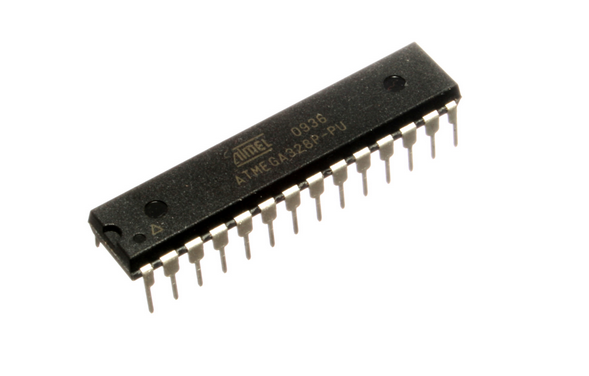
\includegraphics[width = 7 cm]{imagenes/micro.PNG}
    \caption{ATmega 328}
    \cite{atmega}
\end{figure}

\subsubsection{Sensor de obstáculo}
El sensor de obstáculo opera mediante una configuración emisor-receptor de luz infrarroja. Si la luz infrarroja choca contra un obstáculo, esta será reflejada y detectada por el fotodiodo. El rango de detección puede ser configurado mediante los dos controladores. Si no hay un obstáculo en frente la salida del sensor estará en alto, en el momento que se detecte un obstáculo la señal de salida se apagará.

El sensor permite activar o desactivar la detección de obstáculos mediante la manipulación del pin \textit{enable}. Por defecto, el sensor se encuentra en modo activo \cite{obstaculo}.

\begin{figure}[H]
    \centering
    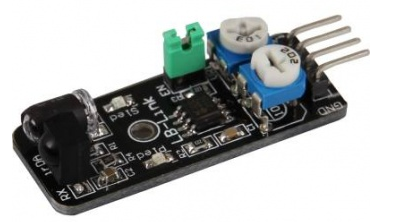
\includegraphics[width = 7 cm]{imagenes/obstacle.PNG}
    \caption{Sensor de obstáculo}
    \cite{obstaculo}
\end{figure}

\subsubsection{Sensor de \textit{traking}}
Es un módulo tipo LEGO, listo para ser conectado al microcontrolador. Se basa en un sensor óptico reflexivo con salida de transistor, el cual se encarga de recibir las señales infrarrojas enviadas para detectar la intensidad de la señal. Con cierto rango de altura, los sensores de pista son ampliamente utilizados para vehículos inteligentes o impresoras para detección de líneas en blanco y negro \cite{track}.

\begin{figure}[H]
    \centering
    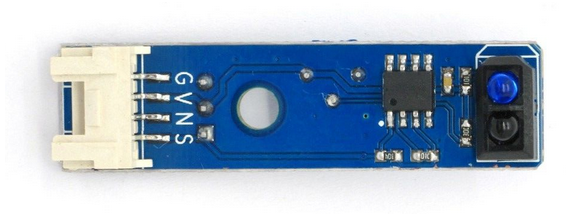
\includegraphics[width = 7 cm]{imagenes/tracking.png}
    \caption{Sensor de pista}
    \cite{track}
\end{figure}


\subsubsection{Motores DC 200 RPM a escala}
Compuesto por un par de motores DC a escala, son usualmente recomendados como una opción barata y sencilla para poner ruedas en movimiento. Requieren una tensión de 4.5V y una corriente sin carga de 190 mA además posee una caja reductora 48:1 y una velocidad de giro de 200 RPM sin carga \cite{motor_dc}.

\begin{figure}[H]
    \centering
    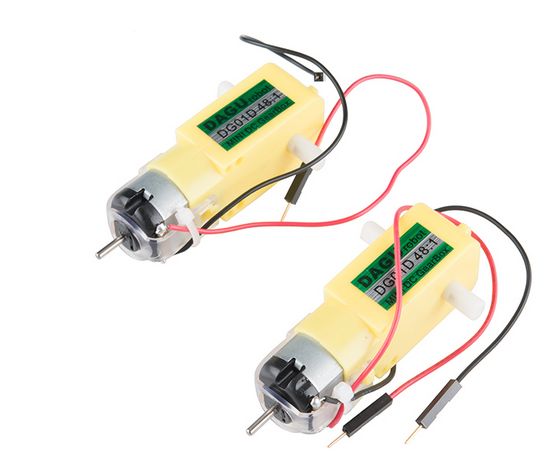
\includegraphics[width = 7 cm]{imagenes/gearmotor.PNG}
    \caption{Hobby Gearmotor - 200 RPM}
    \cite{motor_dc}
\end{figure}

\subsubsection{Módulo de control de motores DC 800 mA}

El módulo de control L9110S 2-Canales es una tarjeta compacta que puede ser utilizada para controlar robots pequeños. Este módulo posee dos controladores independientes capaces de entregar hasta 800 mA en corriente continua. Pueden operar entre 2.5V y 12V lo cual permite que sean usados mediante microcontroladores.

Median de control PWM ---\textit{Pulse Width Modulation}--- es posible controlar la velocidad del motor y una salida digital es usada para indicar la dirección \cite{driver}.

\begin{figure}[H]
    \centering
    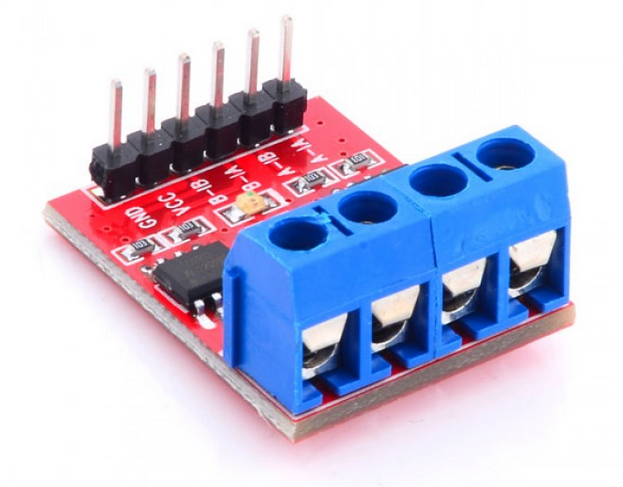
\includegraphics[width = 7 cm]{imagenes/driver.PNG}
    \caption{L9110S Drive Dual Motor DC 800mA}
    \cite{driver}
\end{figure}


\subsubsection{Servomotor}
El servo es un tipo de motor que funciona paso-a-paso, es decir, su giro se determina en ángulos y no en RPM. Pequeño, liviano y con una alta potencia de salida; este tipo de servomotor es capaz de rotar hasta 180 grados \cite{servo}.

\begin{figure}[H]
    \centering
    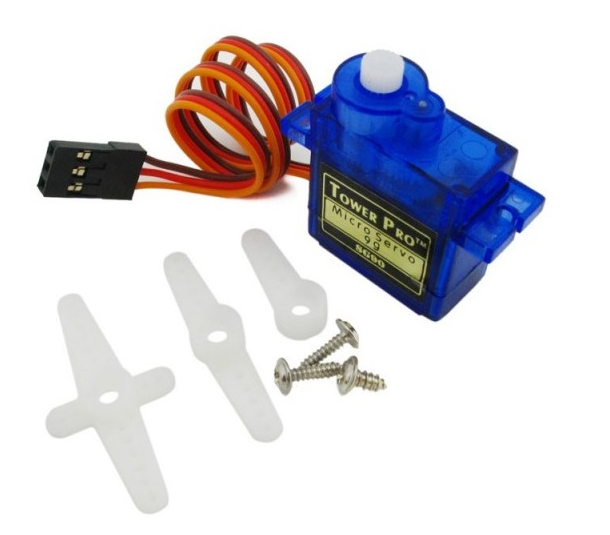
\includegraphics[width = 7 cm]{imagenes/servo.PNG}
    \caption{Servomotor SG90}
    \cite{servo}
\end{figure}

\subsubsection{Piezo Speaker}
Es un pequeño parlante redondo de 12mm el cual opera en todo el rango audible. Pueden ser utilizados para crear interfaces simples musicales. Requiere de una tensión entre los 3.5V y 5V con una corriente media de 35 mA además de una onda cuadrada para su correcto funcionamiento.

\begin{figure}[H]
    \centering
    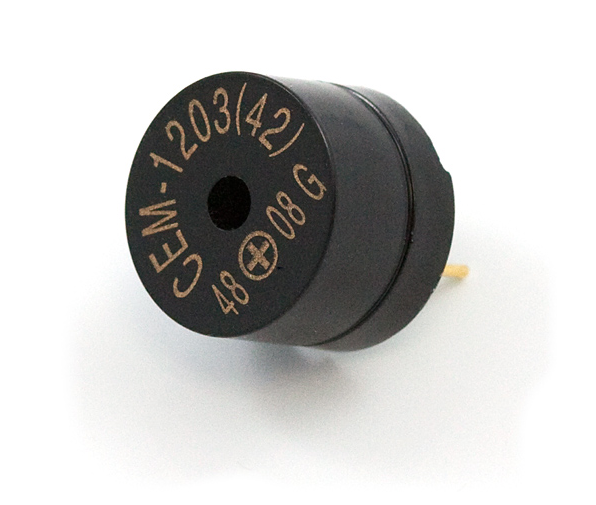
\includegraphics[width = 7 cm]{imagenes/speaker.PNG}
    \caption{Magnetic buzzer}
    \cite{speaker}
\end{figure}


\subsubsection{Módulo bluetooth HC-05}
El módulo bluetooth HC-05 se utiliza en este proyecto para poder enviar datos desde un programa en C al arduino, la comunicación se realiza a través del puerto serial, mediante el cual se transmiten los datos. Dichos datos son interpretados por el arduino para llevar a cabo las funciones que el vehículo realiza. 
\begin{figure}[H]
    \centering
    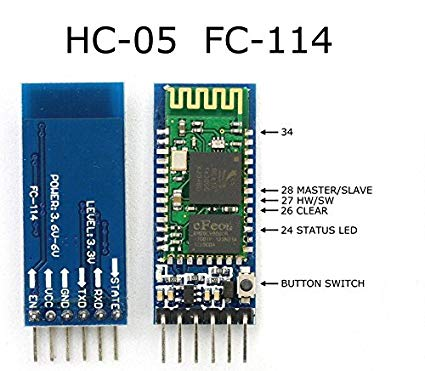
\includegraphics[width= 7 cm]{./imagenes/hc-05.jpg}
    \caption{Módulo bluetooth \cite{bluetooth}}
   
\end{figure}


\subsubsection{Esquemático de conexiones de vehículo}

\begin{figure}[H]
    \centering
    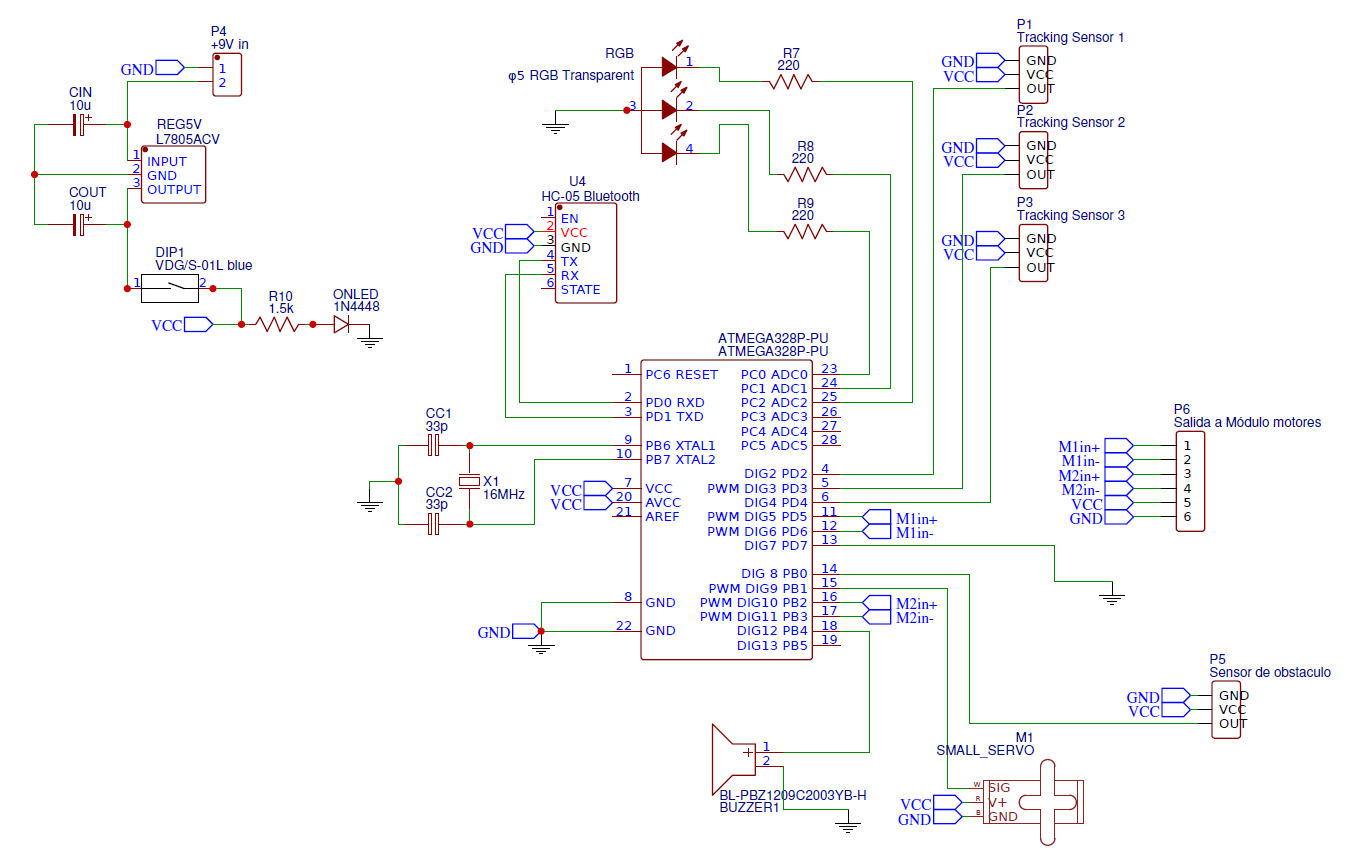
\includegraphics[width = 18 cm]{imagenes/schem_vehiculo.PNG}
    \caption{Esquemático del Vehículo Seguidor de Línea}
\end{figure}




\newpage
\input{Experimentos.tex}
\newpage
\section{Resultados obtenidos}
\subsection{Integración de las funciones en C para Interfaz}
Como se explicó anteriormente, el código utilizado para la creación de la interfaz gráfica, implementa varias funciones que son parte del correcto funcionamiento de la misma. Este permite la combinación de las funciones de GTK y del puerto serial para dar como resultado el control del vehículo de manera inalámbrica, por medio de un módulo \textit{bluetooth} que se puede conectar sin ningún problema con la computadora y así mismo con el código. Por esta razón, al correr el programa se obtiene como resultado la siguiente ventana que corresponde al control del Autonomous Vehicle for Tracking and Control Aplications (AuVeTA):
\begin{figure}[H]
    \centering
    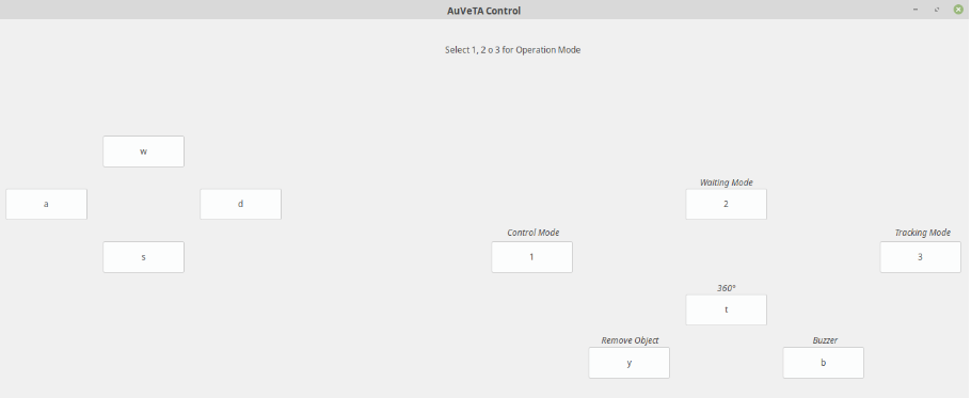
\includegraphics[width = 14cm]{imagenes/interfaz.png}
    \caption{Interfaz Gráfica (Autoría propia)}
    
\end{figure}

\subsection{Implementación del vehículo}
Tras la integración de todos los subsistemas para la conformación del vehículo y la realización de las pruebas correspondientes se produce a efectuar las pruebas críticas finales con el sistema completamente integrado, que implican tanto el funcionamiento del \textit{hardware} como el \textit{software} y las interacciones que existen entre ambos subsistemas. 

Como se ha abordado en la sección 3 de experimentos y pruebas, se obtienen resultados positivos para cada subsistema y además para la integración como un todo. El comportamiento de los sensores de obstáculo y de \textit{tracking} fue el esperado, ya que tanto la detección de objetos para su respectiva remoción como el sensor encargado de enviar la señal indicando el final de la pista y el que detecta la pista en el suelo funcionaron de manera correcta durante la demostración.

Cabe destacar que para la demostración se esperaba contar con una superficie de trabajo clara y regular, pero en el edificio en el que se realizó la demostración el suelo no reunía las condiciones de uniformidad de color necesarias para el funcionamiento del sensor de tracking, por tal motivo se optó por utilizar hojas blancas en el suelo y encima de ellas una cinta de color negro para garantizar el funcionamiento del sensor; ahora bien, este cambio afectó el rodamiento de las llantas y del tercer apoyo por el cambio en la aspereza de la superficie y por tanto además la cantidad de potencia que se utiliza en los motores para el movimiento en el \textit{\´´Tracking Mode"} del vehículo, por lo cual fue necesario realizar una modificación de última hora en el código; el aspecto de modificación de potencia de motores se tenia previsto por lo cual solo fue necesario ajustar una de las variables del código para lograr la modificación de manera rápida y sencilla de la cantidad de potencia enviada a los motores.
\newpage
\section{Conclusiones}
\begin{itemize}
    \item Se logra comprobar con éxito el funcionamiento del vehículo tanto en el modo de control como en el modo de tracking.
    
    \item Se realizaron de manera exitosa las pruebas planteadas en la sección 3 de este documento, esto a pesar de que no se toma en consideración el cálculo de tiempo de autonomía de la fuente de poder con todos los subsistemas en funcionamiento, ya que el tiempo de operación es relativamente corto. No se descarta realizar un pruba de este punto en el futuro con todos los subsistemas trabajando al máximo ciclo de trabajo para determinar la duración de la batería ante condiciones críticas.
     
    \item Se logra la correcta implementación de la interfaz gráfica que permite la comunicación inalámbrica por conexión \textit{bluetooth} con el vehículo.
    
    \item El valor asignado a la potencia del motor para el modo tracking debe ser ajustado dependiendo de la superficie en donde trabaje el vehículo, ya que mucha potencia propiciará que el vehículo se salga de la pista y muy poca hará que aumenten las posibilidades de atascamiento.
    
    \item Para los sensores ópticos se deben considerar las condiciones de luz en el entorno de trabajo y por ello también la calibración de los mismos para garantizar un funcionamiento adecuado y óptimo de los sistemas de control.
     
    \item Se concluye  que se pueden mejorar aspectos constructivos y estéticos de la interfaz para alcanzar un nivel más depurado de experiencia para el usuario. 
\end{itemize}
\newpage
\printbibliography
\newpage
\section{Anexos}

\subsection{Código fuente generado para el Vehículo}
\subsubsection{AuVeTA.ino}
\begin{lstlisting}
/**
 * @file AuVeTA.ino
 * @author Jorge Isaac Fallas Mejía B62562
 * @author Esteban Rodríguez Quintana B66076
 * @brief Archivo de código en arduino para el proyecto final de Programación Bajo Plataformas Abiertas.
 * @version 1.3
 * @date 2019-06-14
 */


/**********include de bibliotecas:************/
#include <Servo.h>          //Servo lib
#include <SoftwareSerial.h> //Bluetooh lib

/******************************************/

/********** Definición de variables: ************/
int RX_bluetooh = 0;
int TX_bluetooh = 1;
int servo_pin = 11;
int obstacle_pin = 8;
int track1_pin = 12;
int final_pin = 7;
int motorR_forward = 9;
int motorR_reverse = 5;
int motorL_forward = 10;
int motorL_reverse = 6;
int buzzer = 13;
int R = 2;
int G = 3;
int B = 4;
int servo_open = 125;  //revisar valores para los grados del servo
int servo_close = 10;  //revisar valores para los grados del servo
int adjustM_delay = 1; //valor cercano a cero
int stopD = 40;        //valor cercano 50
int reactionD = 15;    //entre 10 y 20
int motorPower = 254;

/*  Valores de PWM para variable motorPower:
     _______________________________
    |   Valor   |  Ciclo de trabajo |
    |===============================|
    |    0      |       0%          |
    |    63     |       25%         |
    |    127    |       50%         |
    |    190    |       75%         |
    |    255    |       100%        |
    |_______________________________|
*/

///////////////////////////////////////////////////////
bool obstacle_presence = digitalRead(obstacle_pin); //detección de objeto frontal             // detect = 0 //  no detect = 1  //
bool track1 = digitalRead(track1_pin);              //detección de pista                      // detect = 1 //  no detect = 0  //
bool final_sensor = digitalRead(final_pin);         //detección de objeto lateral             // detect = 0 //  no detect = 1  //


Servo myServo;
SoftwareSerial mySerial(RX_bluetooh, TX_bluetooh); // (RX,TX)

/******************************************/
/*************** SETUP: *******************/
/******************************************/
void setup()
{
  //Seteo para comunicación serial USB:
  Serial.begin(9600);

  ////Seteo para comunicación serial Bluetooth:
  mySerial.begin(115200);

  //Set for digital pins:
  pinMode(R, OUTPUT);
  pinMode(G, OUTPUT);
  pinMode(B, OUTPUT);
  pinMode(servo_pin, OUTPUT);
  pinMode(obstacle_pin, INPUT);
  pinMode(track1_pin, INPUT);
  pinMode(final_sensor, INPUT);
  pinMode(buzzer, OUTPUT);
  pinMode(motorL_forward, OUTPUT);
  pinMode(motorL_reverse, OUTPUT);
  pinMode(motorR_forward, OUTPUT);
  pinMode(motorR_reverse, OUTPUT);

  //Seteo para servo
  myServo.attach(servo_pin);
  myServo.write(servo_close);
  delay(500);
  myServo.detach();
  
  //Seteo inicial de motores en cero
  digitalWrite(motorR_forward, 0);
  digitalWrite(motorL_forward, 0);
  digitalWrite(motorR_reverse, 0);
  digitalWrite(motorL_reverse, 0);
}

/******************************************/
/**************** LOOP: *******************/
/******************************************/
void loop()
{   
//luz roja en "Waiting Mode":
  digitalWrite(R, LOW);
  digitalWrite(G, LOW);
  digitalWrite(B, LOW);
//Revisión de puerto serial disponible
  if (mySerial.available())
  {
//Lectura Serial para selección de modo: 3 -> "Trackig Mode" || 2 -> "Waiting Mode" || 3 -> "Control Mode"
    if (mySerial.read() == '3') //trackin mode
    { //Luz azul para "Tracking Mode":
      digitalWrite(R, LOW);
      digitalWrite(G, HIGH);
      digitalWrite(B, LOW);
      while (1) // "Tracking Mode" hasta cuando el puerto serial recibe un carácter '2' para luego ir a "Waiting Mode"
      {
        tracking_mode_func();
        if (mySerial.read() == '2') //Leer puerto serial para ir a "Waiting Mode"
        {
          break;
        };
      }
    }
    if (mySerial.read() == '1') //Control mode
    { 
      digitalWrite(R, LOW);
      digitalWrite(G, LOW);
      digitalWrite(B, HIGH);
      control_mode_func();    //"Control Mode" hasta cuando el puerto serial recibe un carácter '2' para luego ir a "Waiting Mode"
    }
  }
  else
  {
    while (mySerial.available() == false)
    {
      digitalWrite(R, HIGH);
      delay(100);
      digitalWrite(R, LOW);
      delay(100);
    };
  };

  no_move(); //detener movimiento cuando se esté en modo control y no se precionen teclas.
}

//****************FUNCTIONS: **********************

/**
 * @brief Esta función da movimiento de rueda izquierda y por tanto un giro hacia la derecha del vehículo para el modo de tracking.
 * @param int para potencia deseada en el motor.
 * @return no retorna valores, solo ejecuta acciones.
*/
void goR(int PW)
{
  while (track1 != 1)
  {
    track1 = digitalRead(track1_pin);
    analogWrite(motorR_forward, 0);
    analogWrite(motorL_forward, 0);
    analogWrite(motorR_reverse, 0);
    analogWrite(motorL_reverse, PW);
    delay(adjustM_delay);
    if (mySerial.read() == '2')
    {
      break;
    }
  };

  analogWrite(motorR_forward, 0);
  analogWrite(motorL_forward, 0);
  analogWrite(motorR_reverse, 0);
  analogWrite(motorL_reverse, 0);
  delay(stopD);
};


/**
 * @brief Esta función da movimiento de rueda derecha y por tanto un giro hacia la izquierda del vehículo para el modo de tracking.
 * @param int para potencia deseada en el motor.
 * @return no retorna valores, solo ejecuta acciones.
*/
void goL(int PW)
{
  while (track1 != 0)
  {
    track1 = digitalRead(track1_pin);
    analogWrite(motorR_forward, 0);
    analogWrite(motorL_forward, 0);
    analogWrite(motorR_reverse, PW);
    analogWrite(motorL_reverse, 0);
    delay(adjustM_delay);
    if (mySerial.read() == '2')
    {
      break;
    }
  };
  analogWrite(motorR_forward, 0);
  analogWrite(motorL_forward, 0);
  analogWrite(motorR_reverse, 0);
  analogWrite(motorL_reverse, 0);
  delay(stopD);
}

/**
 * @brief Esta función da movimiento de rueda izquierda y por tanto un giro hacia la derecha del vehículo para el modo de control.
 * @param no recibe parámetros
 * @return no retorna valores, solo ejecuta acciones.
*/
void goR_control()
{
  digitalWrite(motorL_reverse, motorPower);
  digitalWrite(motorL_forward, 0);
  digitalWrite(motorR_reverse, 0);
  digitalWrite(motorR_forward, 0);
  delay(reactionD);
};

/**
 * @brief Esta función da movimiento de rueda derecha y por tanto un giro hacia la izquierda del vehículo para el modo de control.
 * @param no recibe parámetros.
 * @return no retorna valores, solo ejecuta acciones.
*/
void goL_control()
{
  digitalWrite(motorL_reverse, 0);
  digitalWrite(motorL_forward, 0);
  digitalWrite(motorR_reverse, motorPower);
  digitalWrite(motorR_forward, 0);
  delay(reactionD);
};

/**
 * @brief Esta función da movimiento de ambas ruedas en dirección de avance del vehículo para el modo de control.
 * @param no recibe parámetros.
 * @return no retorna valores, solo ejecuta acciones.
*/
void forward_control()
{
  digitalWrite(motorL_reverse, 0);
  digitalWrite(motorL_forward, motorPower);
  digitalWrite(motorR_reverse, 0);
  digitalWrite(motorR_forward, motorPower);
  delay(reactionD);
};

/**
 * @brief Esta función da movimiento de ambas ruedas en dirección contraria al avance del vehículo para el modo de control.
 * @param no recibe parámetros.
 * @return no retorna valores, solo ejecuta acciones.
*/
void reverse_control()
{
  digitalWrite(motorL_reverse, motorPower);
  digitalWrite(motorL_forward, 0);
  digitalWrite(motorR_reverse, motorPower);
  digitalWrite(motorR_forward, 0);
  delay(reactionD);
};

/**
 * @brief Esta función apaga motores del vehículo para el modo de control.
 * @param no recibe parámetros.
 * @return no retorna valores, solo ejecuta acciones.
*/
void no_move()
{
  digitalWrite(motorL_reverse, 0);
  digitalWrite(motorL_forward, 0);
  digitalWrite(motorR_reverse, 0);
  digitalWrite(motorR_forward, 0);
};

/**
 * @brief Esta función determina si se detecta el final del recorrido gracias a la condición recibida de un sensor de tracking y otro de obstáculo.
 * @param Recibe el valor del sensor de tracking.
 * @param Recibe el valor del sensor de obstáculo lateral.
 * @return Retorna un bool que indica si el final de la pista ha sido alcanzado.
*/
bool end_detection(int _track1, int _track2)
{
  bool FINAL_DE_PISTA = false;
  if ((_track1 == 1) && (_track2 == 0))
  {
    FINAL_DE_PISTA = true;
  }
  return FINAL_DE_PISTA;
};



/**
 * @brief Esta función determina si se detecta un obstáculo frontal gracias al sensor de obstáculo, en caso de presencia de obstáculo activa el servomotor para removerlo..
 * @param Recibe el valor de un sensor de obstáculo frontal.
 * @return No retorna valores, solo activa el servomotor.
*/
void obstacle_detection(bool _obstacle_presence)
{
  if (_obstacle_presence == 0)
  {
    myServo.attach(servo_pin);
    myServo.write(servo_open);
    delay(700);
    myServo.write(servo_close);
    delay(700);
  };
  myServo.detach();
}



/**
 * @brief Esta función solo enciende las luces en una determinada secuencia para indicar el final del recorrido.
 * @param No recibe parámetros.
 * @return No retorna, solo acciona LED RGB.
*/
void final_track_indicator()
{
  digitalWrite(R, HIGH);
  delay(100);
  digitalWrite(R, HIGH);
  delay(50);
  digitalWrite(G, HIGH);
  delay(100);
  digitalWrite(G, LOW);
  delay(50);
  digitalWrite(B, HIGH);
  delay(100);
  digitalWrite(B, LOW);
  delay(50);
  digitalWrite(R, HIGH);
  delay(100);
  digitalWrite(R, HIGH);
  delay(50);
  digitalWrite(G, LOW);
  delay(100);
  digitalWrite(G, LOW);
  delay(50);
  digitalWrite(B, HIGH);
  delay(100);
  digitalWrite(B, LOW);
  digitalWrite(R, LOW);
  digitalWrite(G, LOW);
  delay(100);
};


/**
 * @brief Esta función hace que se activen las ruedas de manera que el vehíulo gire sobre su propio eje horizontal para el modo tracking.
 * @param No recibe parámetros.
 * @return No retorna.
*/
void trompo()
{
  digitalWrite(motorL_reverse, motorPower);
  digitalWrite(motorL_forward, 0);
  digitalWrite(motorR_reverse, 0);
  digitalWrite(motorR_forward, motorPower);
  delay(reactionD);
};

/**
 * @brief Esta función hace que se activen las ruedas de manera que el vehíulo gire sobre su propio eje horizontal para el modo control.
 * @param Recibe la potencia que se desea usar para los motores.
 * @return No retorna.
*/
void trompo_final(int power)
{
  digitalWrite(motorL_reverse, power);
  digitalWrite(motorL_forward, 0);
  digitalWrite(motorR_reverse, 0);
  digitalWrite(motorR_forward, power);
};

/**
 * @brief Esta función implementa y ejecuta las acciones y funciones necesarias para el funcionamiento durante el modo tracking.
 * @param No recibe parámetros.
 * @return No retorna.
*/
void tracking_mode_func()
{
  goL(235);
  goR(235);
  obstacle_detection(digitalRead(obstacle_pin));
  if (end_detection(digitalRead(track1_pin), digitalRead(final_pin)) == 1)      // if structure to check final of track
  {
    delay(1000);
    while (1)
    {
      trompo_final(200);
      delay(300);
      trompo_final(0);
      delay(100);
      final_track_indicator();
      if (mySerial.read() == '2')   //break cuando el puerto serial recibe un carácter '2' y luego se va a "Waiting Mode"
      {
        break;
      };
    }
  };
};


/**
 * @brief Esta función implementa y ejecuta las acciones y funciones necesarias para el funcionamiento durante el modo de control.
 * @param No recibe parámetros.
 * @return No retorna.
*/
void control_mode_func()
{
  char c;
  while (1)
  {
    no_move();
    c = mySerial.read();    //actualización constante para valor recibido en puerto serial
    if (c == 's') //Reverse
    {
      forward_control();
    };
    if (c == 'w') //forward
    {
      reverse_control();
    };
    if (c == 'a') //Turn left
    {
      goL_control();
    };
    if (c == 'd') //Turn rigth
    {
      goR_control();
    };
    if (c == 'b') //buzzer sound
    {
      digitalWrite(buzzer, HIGH);
      delay(1);
      digitalWrite(buzzer, LOW);
      delay(1);
      digitalWrite(buzzer, HIGH);
      delay(1);
    };
    if (c == 't') //trompo
    {
      trompo();
    };
    if (c == '2') //break cuando el puerto serial recibe un carácter '2' y luego se va a "Waiting Mode"
    {
      break;
    };
    if (c == 'y') //Obstacle remove
    {
      myServo.attach(servo_pin);
      myServo.write(servo_open);
      delay(700);
      myServo.write(servo_close);
      delay(700);
      myServo.detach();
    };
  }
};

\end{lstlisting}
\newpage
\subsection{Código fuente generado para Interfaz y Comunicación Serial}

\subsubsection{h\_comunicación\_interfaz.h}
\begin{lstlisting}
/**
 * @file h_comunicación_interfaz.h
 * @author Jorge Isaac Fallas Mejía B62562
 * @author Esteban Rodríguez Quintana B66076
 * @author Fabio Villalobos Pacheco B78346
 * @brief Archivo de encabezado para la interfaz y la comunicación
 * @version 1
 * @date 2019-07-18
 *
 *
 */
#ifndef A
#define A

#include <stdio.h> /* Standard input/output definitions */
#include <stdlib.h>
#include <stdint.h>  /* Standard types */
#include <string.h>  /* String function definitions */
#include <unistd.h>  /* UNIX standard function definitions */
#include <fcntl.h>   /* File control definitions */
#include <errno.h>   /* Error number definitions */
#include <termios.h> /* POSIX terminal control definitions */
#include <sys/ioctl.h>
#include <getopt.h>
#include <gtk/gtk.h>

#define BUF_SIZE 88
static float num1 = 0;
static char lastChar = (char)0;
static char prevCmd = (char)0;
/**
 * @brief Estructura de datos para realizar un seguimiento de los botones de la interfaz.
 */

typedef struct {

        char *szLabel;
        int row;
        int col;
        GtkWidget *widget;

} MoButton;

/**
 * @brief Lista MoButton: Crea una lista que contendrá los botones que aparecerán en la interfaz gráfica.
 */

MoButton * buttonList;

/**
 * @brief int numbuttons: Es la variable de tipo entero que contiene el número de botones que estarán en
 * la lista MoButton.
 */

int numbuttons;

/**
 * @brief Widget label: Este es el panel en el que se "imprime" la función de los botones.
 *
 */

GtkWidget *label;

/*Funciones comunicación serial*/
/**
 *@brief Función serialport_init: Inicializa el puerto serial.
 *@param serialport: El nombre del puerto al que se conecta el módulo bluetooth.
 *@param baud: El baud rate que utiliza el módulo bluetooth.
 *@return int: Si el puerto pudo ser inicializado.
*/
int serialport_init(const char *serialport, int baud);
/**
 *@brief Función serialport_write: Escribe en el puerto serial.
 *@param fd: La función serialport_init.
 *@param str: El caracter que se envía en el puerto.
 *@return int: El dato enviado por el puerto.
*/
int serialport_write(int fd, const char *str);


/* Funciones GTK */
/**
 * @brief Función CloseAppWindow: Cierra la ventana creada de la interfaz.
 * @param widget: La "caja" que contiene el texto del botón.
 * @param data: El puntero del texto contenido en el "widget".
 * @return FALSE: Retorna el cierre de la ventana del programa y finalización de operación.
 */
gint CloseAppWindow (GtkWidget *widget, gpointer data);

/**
 * @brief Función key_press: Se encarga de la lectura del botón presionado en el teclado.
 * @param widget: La "caja" que contiene el texto del botón.
 * @param event: El evento que lee el botón presionado.
 * @param data: El puntero del texto contenido en el "widget".
 * @return Retorna la tarea del botón presionado.
 */
void key_press(GtkWidget *widget, GdkEventKey *event, gpointer data);

/**
 * @brief Función button_clicked: Se encarga de leer que el botón en la interfaz se haya clickeado.
 * @param widget: La "caja" que contiene el texto del botón.
 * @param data: El puntero del texto contenido en el "widget".
 * @return Retorna la tarea del botón clickeado.
 */
void button_clicked (GtkWidget *widget, gpointer data);

/**
 * @brief Función CreateButton: Se encarga de crear las características de cada botón.
 * @param table: La tabla que contiene los botones.
 * @param szLabel: El tamaño del texto que contiene el botón.
 * @param row: La fila donde se ubicará el botón.
 * @param column: La columna donde se ubicará el botón.
 * @return button: Retorna el botón creado.
 */
GtkWidget *CreateButton (GtkWidget *table, char *szLabel, int row, int column);

/**
 * @brief Función CreateControlButtons: Se encarga de poner en la interfaz los botones que se crearon.
 * @param table: La tabla que contiene los botones.
 * @return Retorna los botones en la interfaz.
 */
void CreateControlButtons (GtkWidget *table);
#endif


\end{lstlisting}
\newpage
\subsubsection{comunicación\_interfaz.c}
\begin{lstlisting}
/**
 * @file comunicación_interfaz.c
 * @author Jorge Isaac Fallas Mejía B62562
 * @author Esteban Rodríguez Quintana B66076
 * @author Fabio Villalobos Pacheco B78346
 * @brief Archivo de funciones para la interfaz y la comunicación
 * @version 1
 * @date 2019-07-18
 *
 *
 */
#include "h_comunicación_interfaz.h"

/**
 * @brief int CloseAppWindow: Es una función de tipo int que
 * recibe un widget y la información, que utiliza un
 * gtk_main_quit que retorna el cierre de la ventana y, por
 * ende, del programa.
 */
int CloseAppWindow(GtkWidget *widget, gpointer data)
{
        gtk_main_quit();

        return (FALSE);
}

/**
 * @brief void key_press: Es una función de tipo void que recibe
 * un widget, un evento y la información, hace uso de un ciclo
 * for que busca entre los botones, y una condición if que si la
 * pulsación de tecla es el primer carácter de un botón y la longitud
 * de la etiqueta del botón es uno, entonces permite el retorno que
 * conecta el botón presionado en el teclado con la interfaz gráfica
 * tarea asociada.
 */

void key_press(GtkWidget *widget,
               GdkEventKey *event,
               gpointer data)
{
        int npressed;

        for (npressed = 0; npressed < numbuttons; npressed++)
        {
                if (event->keyval == buttonList[npressed].szLabel[0] &&
                    buttonList[npressed].szLabel[1] == (char)0)
                {
                        gtk_widget_grab_focus(buttonList[npressed].widget);

                        gtk_button_clicked(GTK_BUTTON(buttonList[npressed].widget));
                        return;
                }
        }
}

/**
 * void button_clicked: Es una función de tipo void que recibe un widget
 * y la información, este contiene instancias de las funciones que trabajan
 * con el puerto serial, dos punteros de tipo char, el str se encarga
 * de agarrar el texto del botón y la información, además contiene
 * la ventana que contiene la interfaz, luego varias condiciones if
 * que permiten comparar el botón clickeado o presinado en el teclado
 * que conecta con el puerto serial y retorna la tarea que realiza
 * el vehículo.
 */

void button_clicked(GtkWidget *widget, gpointer data)
{
        int baudrate = 115200;
        int port;
        port = serialport_init("/dev/rfcomm0", baudrate);

        char ch = *((char *)data);
        char *str;
        GtkWidget *window;
        window = gtk_window_new(GTK_WINDOW_TOPLEVEL);

        str = (char *)data;

        if (strcmp(str, "w") == 0)
        {

                char a = 'w';
                const char *ptr = &a;
                serialport_write(port, ptr);

                return;
        }
        else if (strcmp(str, "a") == 0)
        {

                char a = 'a';
                const char *ptr = &a;
                serialport_write(port, ptr);

                return;
        }
        else if (strcmp(str, "d") == 0)
        {

                char a = 'd';
                const char *ptr = &a;
                serialport_write(port, ptr);

                return;
        }
        else if (strcmp(str, "s") == 0)
        {

                char a = 's';
                const char *ptr = &a;
                serialport_write(port, ptr);

                return;
        }
        else if (strcmp(str, "1") == 0)
        {

                char a = '1';
                const char *ptr = &a;
                serialport_write(port, ptr);

                gtk_label_set(GTK_LABEL(label), "Control Mode");
                return;
        }
        else if (strcmp(str, "2") == 0)
        {

                char a = '2';
                const char *ptr = &a;
                serialport_write(port, ptr);

                gtk_label_set(GTK_LABEL(label), "Waiting mode");
                return;
        }
        else if (strcmp(str, "3") == 0)
        {

                char a = '3';
                const char *ptr = &a;
                serialport_write(port, ptr);

                gtk_label_set(GTK_LABEL(label), "Tracking mode");
                return;
        }
        else if (strcmp(str, "y") == 0)
        { //scalubur time

                char a = 'e';
                const char *ptr = &a;
                serialport_write(port, ptr);

                return;
        }
        else if (strcmp(str, "b") == 0)
        { //buzzer

                char a = 'b';
                const char *ptr = &a;
                serialport_write(port, ptr);

                return;
        }
        else if (strcmp(str, "t") == 0)
        { //trompo

                char a = 't';
                const char *ptr = &a;
                serialport_write(port, ptr);

                return;
        }


}

/**
 * @brief GtkWidget *CreateButton: Es una función tipo Gtkwidget
 * que recibe la tabla que contiene los botones, un dato
 * char que es el tamaño de los botones, además dos datos de
 * tipo int que son la posición en fila y columna de los botones,
 * luego esta hace un gtk_button_new_with_label que es el botón,
 * además del color, de la posicion en la interfaz y gtk_widget_show
 * que hace que retorne todas esas características del botón.
 */

GtkWidget *CreateButton(GtkWidget *table, char *szLabel, int row, int column)
{
        GtkWidget *button;

        button = gtk_button_new_with_label(szLabel);

        gtk_signal_connect(GTK_OBJECT(button), "clicked",
                           GTK_SIGNAL_FUNC(button_clicked), szLabel);

        GdkColor color;

        gdk_color_parse("red", &color);

        gtk_widget_modify_bg(GTK_WIDGET(button), GTK_STATE_NORMAL, &color);

        gtk_table_attach(GTK_TABLE(table), button,
                         column, column + 1,
                         row, row + 1,
                         GTK_FILL | GTK_EXPAND,
                         GTK_FILL | GTK_EXPAND,
                         10, 15);

        gtk_widget_show(button);

        return (button);
}

/**
 * @brief void CreateControlButtons: Es una función tipo void
 * que recibe la tabla que contiene los botones, luego se crea
 * un dato que hace que el ciclo for recorra la lista de los
 * botones y con ayuda de la función CreateButton se cree el
 * botón y aparezca en la interfaz.
 */

void CreateControlButtons(GtkWidget *table)
{
        int nIndex;

        for (nIndex = 0; nIndex < numbuttons; nIndex++)
        {

                buttonList[nIndex].widget =
                    CreateButton(table,
                                 buttonList[nIndex].szLabel,
                                 buttonList[nIndex].row,
                                 buttonList[nIndex].col);
        }
}

/////////////////////////////////////////////////////
/**
 *@brief Función serialport_write: Esta función recibe de parámetros el puerto
 *inicializado y el caracter que se desea enviar. Luego, el caracter se escribe
 *en el puerto inicializado para ser recibido en el arduino.
*/

int serialport_write(int fd, const char *str)

{

        int len = strlen(str);

        int n = write(fd, str, len);

        if (n != len)

                return -1;

        return n;
}
/**
 *@brief Función serialport_init: Esta función recibe de parámetros el nombre
 *del puerto que se desea inicializar y el baud rate que utiliza el módulo bluetooth.
 *Seguidamente, el puerto es abierto para poder escribir o leer datos.
*/

int serialport_init(const char *serialport, int baud)

{

        int fd;
        fd = open(serialport, O_RDWR | O_NOCTTY);
        if (fd == -1)
        {

                perror("init_serialport: Unable to open port ");

                return -1;
        }
        return fd;
}


\end{lstlisting}
\newpage
\subsubsection{main.c}
\begin{lstlisting}
/**
 * @file main.c
 * @author Jorge Isaac Fallas Mejía B62562
 * @author Esteban Rodríguez Quintana B66076
 * @author Fabio Villalobos Pacheco B78346
 * @brief Archivo de código main para el proyecto AuVeTA
 * @version 1
 * @date 2019-07-18
 *
 *
 */

#include "h_comunicación_interfaz.h"

int main(int argc, char *argv[])
{

	numbuttons = 10;
	buttonList = malloc(sizeof(MoButton) * 11);

	int i = 0;
	buttonList[i++] = (MoButton){"w", 2, 1, NULL};
	buttonList[i++] = (MoButton){"a", 3, 0, NULL};
	buttonList[i++] = (MoButton){"d", 3, 2, NULL};
	buttonList[i++] = (MoButton){"s", 4, 1, NULL};
	buttonList[i++] = (MoButton){"1", 4, 5, NULL};
	buttonList[i++] = (MoButton){"2", 3, 7, NULL};
	buttonList[i++] = (MoButton){"3", 4, 9, NULL};
	buttonList[i++] = (MoButton){"y", 6, 6, NULL};
	buttonList[i++] = (MoButton){"t", 5, 7, NULL};
	buttonList[i++] = (MoButton){"b", 6, 8, NULL};

	GtkWidget *window;
	GtkWidget *table;

	/* --- GTK initialization --- */
	gtk_init(&argc, &argv);

	/* --- Create the AuVeTA Control window --- */
	window = gtk_window_new(GTK_WINDOW_TOPLEVEL);

	/* --- Give the window a title. --- */
	gtk_window_set_title(GTK_WINDOW(window), "AuVeTA Control");

	/* --- Set the window size. --- */
	gtk_widget_set_usize(window, 1000, 700);

	/* --- We care if a key is pressed --- */
	gtk_signal_connect(GTK_OBJECT(window), "key_press_event",
					   GTK_SIGNAL_FUNC(key_press), NULL);

	/* --- You should always remember to connect the delete event
         *     to the main window. --- */
	gtk_signal_connect(GTK_OBJECT(window), "delete_event",
					   GTK_SIGNAL_FUNC(CloseAppWindow), NULL);

	/* --- Create a 10x10 table for the items in the control. --- */
	table = gtk_table_new(10, 10, TRUE);

	/* --- Create the control buttons. --- */
	CreateControlButtons(table);

	/* --- Create the label --- */



	label = gtk_label_new (NULL);
	const char *str1 = "Control Mode";
	const char *format1 = "<span style=\"italic\">%s</span>" ;
	char *markup1;

	markup1 = g_markup_printf_escaped (format1, str1);
	gtk_label_set_markup (GTK_LABEL (label), markup1);

	gtk_misc_set_alignment(GTK_MISC(label), 0.96, .58);
	/* --- Add label to the table --- */
	gtk_table_attach_defaults(GTK_TABLE(table), label, 0, 6, 0, 7);

	gtk_widget_show(label);

	g_free (markup1);

	/* --- Create the label --- */
	label = gtk_label_new (NULL);
	const char *str2 = "Waiting Mode";
	const char *format2 = "<span style=\"italic\">%s</span>" ;
	char *markup2;

	markup2 = g_markup_printf_escaped (format2, str2);
	gtk_label_set_markup (GTK_LABEL (label), markup2);

	gtk_misc_set_alignment(GTK_MISC(label), 0.97, .44);


	/* --- Add label to the table --- */
	gtk_table_attach_defaults(GTK_TABLE(table), label, 0, 8, 0, 7);

	gtk_widget_show(label);

	g_free (markup2);


	/* --- Create the label --- */
	label = gtk_label_new (NULL);
	const char *str3 = "Tracking Mode";
	const char *format3 = "<span style=\"italic\">%s</span>" ;
	char *markup3;

	markup3 = g_markup_printf_escaped (format3, str3);
	gtk_label_set_markup (GTK_LABEL (label), markup3);

	gtk_misc_set_alignment(GTK_MISC(label), 0.98, .58);
	/* --- Add label to the table --- */
	gtk_table_attach_defaults(GTK_TABLE(table), label, 0, 10, 0, 7);

	gtk_widget_show(label);

	g_free (markup3);

	/* --- Create the label --- */
	label = gtk_label_new (NULL);
	const char *str4 = "Remove Object";
	const char *format4 = "<span style=\"italic\">%s</span>" ;
	char *markup4;

	markup4 = g_markup_printf_escaped (format4, str4);
	gtk_label_set_markup (GTK_LABEL (label), markup4);

	gtk_misc_set_alignment(GTK_MISC(label), 0.97, .61);
	/* --- Add label to the table --- */
	gtk_table_attach_defaults(GTK_TABLE(table), label, 0, 7, 0, 10);

	gtk_widget_show(label);

	g_free (markup4);

	/* --- Create the label --- */
	label = gtk_label_new (NULL);
	const char *str5 = "360°";
	const char *format5 = "<span style=\"italic\">%s</span>" ;
	char *markup5;

	markup5 = g_markup_printf_escaped (format5, str5);
	gtk_label_set_markup (GTK_LABEL (label), markup5);

	gtk_misc_set_alignment(GTK_MISC(label), 0.949, .51);
	/* --- Add label to the table --- */
	gtk_table_attach_defaults(GTK_TABLE(table), label, 0, 8, 0, 10);

	gtk_widget_show(label);

	g_free (markup5);

	/* --- Create the label --- */
	label = gtk_label_new (NULL);
	const char *str6 = "Buzzer";
	const char *format6 = "<span style=\"italic\">%s</span>" ;
	char *markup6;

	markup6 = g_markup_printf_escaped (format6, str6);
	gtk_label_set_markup (GTK_LABEL (label), markup6);

	gtk_misc_set_alignment(GTK_MISC(label), 0.96, .61);
	/* --- Add label to the table --- */
	gtk_table_attach_defaults(GTK_TABLE(table), label, 0, 9, 0, 10);

	gtk_widget_show(label);

	g_free (markup6);

	/* --- Create the label --- */
	label = gtk_label_new("Select 1, 2 o 3 for Operation Mode");
	gtk_misc_set_alignment(GTK_MISC(label), 2, .6);

	/* --- Add label to the table --- */
	gtk_table_attach_defaults(GTK_TABLE(table), label, 0, 6, 0, 1);
	gtk_widget_show(label);

	/* --- Make LABELS  visible --- */
	gtk_container_add(GTK_CONTAINER(window), table);
	gtk_widget_show(table);

	gtk_widget_show(window);

	/* --- Grab focus for the keystrokes --- */
	//gtk_widget_grab_focus (buttonList[0].widget);

	gtk_main();
	free(buttonList);
	return (0);
}


\end{lstlisting}
\subsubsection{Makefile}

\begin{lstlisting}
SRC_DIR = ./src
INCLUDE_DIR = ./incl
BIN_DIR = ./bin
DOC_DIR = ./doc
CFLAGS =

BIN_OUT = Carrito.out

CC = gcc

build:
	mkdir --parents $(BIN_DIR)
	$(CC) -I $(INCLUDE_DIR) $(SRC_DIR)/comunicación_interfaz.c main.c  -o $(BIN_DIR)/$(BIN_OUT) `pkg-config --cflags --libs gtk+-2.0` -lm

run:
	./$(BIN_DIR)/$(BIN_OUT)

clean:
	rm -rf $(BIN_DIR)/$(BIN)
	rm -rf doc

doc:
	doxygen ./Doxyfile
	cd doc/latex && make


\end{lstlisting}
\end{document}

